\documentclass{article}

\usepackage{titlesec}
\usepackage{graphicx}
\usepackage{amsmath}
\usepackage{amssymb}
\usepackage{float}
\usepackage{hyperref}
\usepackage[zihao=-4]{ctex}
\usepackage[a4paper]{geometry}
\usepackage{ragged2e} % ragged2e 宏包用来设置左右对齐
\usepackage{parskip} % parskip 宏包用来设置段落间距和首行缩进
\usepackage{subcaption}
\usepackage{array}
\usepackage{ctex}
\usepackage{booktabs}
\usepackage{tikz}
\usepackage{pgfplots}
\usepackage{listings}

\setlength{\parindent}{2em} % 设置首行缩进为2个字符
\setCJKmainfont{SimSun} % 设置宋体字体

% 设置文档行间距为1.15倍
\renewcommand{\baselinestretch}{1.15}

% 设置页边距
\geometry{left=2.54cm,right=2.54cm,top=3.17cm,bottom=3.17cm}

% Title
\title{\textbf{基于大学生餐厅消费数据的隐性资助模型\\——揭示经济贫困学生的精准援助之路}}
\date{} % 删除日期

\begin{document}
\maketitle

% Abstract
\begin{abstract}
本文介绍了一种基于大学生餐厅消费数据的隐性资助模型。在当今社会中,精确资助的重要性越来越明显。
尤其对于高校中的经济困难学生而言,准确地识别并提供有效援助是当前高等教育贫困援助工作的关键问题。通过利用大数据技术,
我们对大学生的餐厅消费数据进行了统计和分析,并建立了隐性资助模型。该模型能够根据学生的消费数据评估其经济贫困程度,
从而实现精准援助,为教育扶贫事业提供支持。

在构建模型之前,在构建模型之前,考虑到某些用餐时段有非自然原因造成的数据可信度低,我们首先筛除消费人数少于1000的用餐时间(列数).
得到精简数据后,我们使用 PCA 对两类数据进行特征提取,总计提取到 20 余个特征维度,以便后续的模型构建与训练等。

对于问题1,本文使用K-Means算法,通过设置K值为3来将第一学年的学生分为三类,以消费水平(消费稳定性)为划分标准。然后本文计算了三类学生各自的
三年的消费特征的均值,并绘制图表来更加直观地体现消费特征的变化。最后发现这些学生的消费能力在提高,消费习惯也变得更加稳定。

对于问题2,本文通过分析,采用XGBoost模型,并使用交叉验证、启发式算法寻优来提高模型的精度,利用已知数据对全体同学二三学年的贫困程度进行预测,
预测效果良好。

对于问题3,通过将第二类附件提取出的特征数据作为新的指标放入模型进行训练,进一步将模型精度提高了16.22\%。

对于问题4,我们采用熵权法对第三学年学生的各个指标进行权重赋值,并进行综合评价,计算他们的综合得分。
根据每个学生的贫困程度得分,我们使用线性插值方法来确定贫困程度排名前80位的同学的资助金额分配。
最终,贫困程度排名第一的同学被分配了2537元的资助金额,而排名第80的同学被分配了200元的资助金额。

总之,基于大学生餐厅消费数据的隐形资助模型充分体现了大数据时代的特点,并且在教育援助方面注重了准确性和公平性。
同时,该模型也尊重了学生的隐私权,真正关注每个学生的需求,体现了以人为本的理念。因此,这种模型具有广阔的应用前景,
值得我们进行深入的探讨和研究。

\textbf{关键词:} PCA数据降维,K-Means聚类,XGBoost模型,熵权法。
\end{abstract}

% Main Content
\section{问题重述}

\subsection{问题背景}

随着精准资助在高校的推进,准确判定经济困难学生并改进资助手段变得非常重要。隐性资助通过大数据挖掘的方式,利用学生的行为和经济特征,
以隐蔽的方式认定困难学生并给予适度的资助,以保护学生的隐私并促进教育公平。信息化水平的提高使得学生的一些消费数据,例如食堂三餐消费,
可以有效记录和留存。这些消费数据,如消费金额、消费次数等,被认为可以间接反映学生的经济状况。在这个背景下,某管理部门模拟了一组学生的消费数据。

针对这些数据,需要建立数学模型来挖掘不同代表性群体,并定量分析这些群体在三个学年中的主要消费行为特征变化规律以及饮食种类变化规律等。
数据预处理(如删除不相关数据、补全缺失数据、提取特征等)是建模前必要的步骤。

除了上述信息,附件8提供了部分同学在第一学年后通过其他方式认定的贫困程度等级(粗粒度)。请建立数学模型根据消费行为(附件1-3)预测贫困程度
,并补全附件9的数据,保持附件9的已有数据和顺序不变。结合第一问的研究结果,进一步预测该组同学在第二和第三学年的贫困程度隐性认定等级,并分析相关变化。

在第二问的基础上,结合附件4-7中的饮食种类数据,改进预测模型,比较分析相关同学的预测结果的变化情况。

通过挖掘贫困生的本质特征,构建差异化的资助额度分配算法,并以第三学年为例给出具体结果。目标对象为附件4-7中涉及的同学,
资助总金额为10万,资助人员为80名,并评估资助结果的公平合理性。

\subsection{问题重述}

在高校精准资助的背景下,需要建立数学模型来准确判定经济困难学生并改进资助手段。该模型基于大数据挖掘学生的消费数据,
特别是餐厅消费数据,以隐性方式识别困难学生并给予适度的资助。具体问题包括:

1. 针对给定的学生消费数据,建立模型分析不同学年的主要消费行为特征变化和饮食种类变化规律。

2. 利用消费行为数据预测学生的贫困程度,并补全附件中的贫困程度数据。结合第一问题的结果,
预测学生在第二和第三学年的贫困程度隐性认定等级,并分析相关变化。

3. 结合饮食种类数据,改进贫困程度预测模型,并比较分析预测结果的变化情况。

4. 基于贫困生的本质特征挖掘,构建差异化的资助额度分配算法。以第三学年为例,给出具体的资助结果,包括涉及的同学、
资助总金额和资助人员数量,并评估资助结果的公平合理性。

\section{问题分析与模型假设}

\subsection{问题分析}

首先,先对所给数据作特征提取和数据降维。从附件1-3中提取全体学生三年的消费特征,从附件4-7中提取出部分学生的消费金额特征以及食物种类特征,以便后续的模型训练。

问题一的分析将采用K-Means算法对第一学年的学生进行聚类,并计算三年消费特征的均值,以图形形式展示相关变化。
这种方法具有显著的优势,因为K-Means算法是一种被广泛应用的聚类算法,可以有效地识别具有相似消费行为特征的学生群体。
通过计算三年消费特征的均值,可以量化和比较不同学年的消费行为变化,从而揭示出主要的消费行为特征变化规律。

绘制图形是一种直观而有效的方法,以图形形式呈现聚类结果和消费特征变化。
通过图形,可以清晰地观察不同学年的消费行为模式是否存在明显差异,以及哪些特征对变化起到主导作用。
这样的分析有助于深入了解学生的消费行为特征,并为精准资助提供更具针对性的建议和决策依据。

问题二的分析涉及构建XGBoost模型,并使用交叉验证和启发式算法进行模型优化,以提高预测的准确性。
在模型训练过程中,将利用附件8的数据作为训练集,对附件9中的同学进行贫困程度的预测。此外,还将对全体同学在第二和第三学年的贫困程度进行预测。

采用XGBoost模型是合理的选择,因为XGBoost是一种强大且广泛应用于预测和分类问题的机器学习算法。它能够处理复杂的数据关系,
并具有较高的预测准确性。同时,使用交叉验证和启发式算法寻优可以进一步提升模型的性能,确保预测结果更加准确和可靠。

通过使用附件8的数据进行模型训练,我们可以建立一个贫困程度预测模型,并将其应用于附件9中的同学进行预测。这将帮助我们更好地了解学生的贫困程度,
并为精准资助提供定量的依据。
此外,对全体同学在第二和第三学年的贫困程度进行预测是一个重要的任务。通过该预测,我们能够观察贫困程度随时间的变化趋势,
揭示学生经济状况的发展轨迹,并为资助决策提供长期的规划和参考。

问题三的分析中,计划将从附件4-7中提取到的新特征与原有指标一起纳入模型的指标体系,以提高预测的准确性。

将附件4-7中提取到的新特征纳入模型的指标体系是一个合理而重要的步骤。这些新特征可能包含与学生饮食种类相关的信息,
这对于预测学生的贫困程度可能起到关键作用。通过将这些特征与原有指标一起考虑,可以综合考虑更多的因素,提高模型的预测能力。

这一分析方法能够更全面地捕捉学生的消费行为特征和饮食种类,为贫困程度的预测提供更多的信息和线索。同时,
通过比较和分析附件4-7中的新特征对预测结果的影响,我们可以评估这些特征的重要性和贡献度,进一步优化模型的指标体系。\cite{reference5,reference6}

\subsection{模型假设}

\begin{enumerate}
  \item 假设本文数据挖掘及处理研究过程中只有系统误差,无随机误差;假设本文所研究的各项因素的误差是不相关的。
  \item 假设学生的贫困程度在一定时间范围内相对稳定,即在短期内贫困程度变化较小.
  \item 假设每位同学的餐厅消费记录均为本人真实消费记录,不存在他人代刷的情况,数据真实有效完整。
  \item 假设所有学生得到的资助仅与学生贫困程度有关,与其他外部因素无关。
  \item 假设模型训练数据与实际应用数据具有一定的代表性和稳定性,即模型在实际应用中的表现与训练时的性能相当。
\end{enumerate}

\section{数据预处理及PCA数据降维}

\subsection{无效数据剔除}

考虑到在给出的数据中也包括寒暑假等部分“异常时间段”,其会影响模型的训练效果和准确性,故本文先把有问题的“无效”数据进行剔除。

该做法的动机是,我们发现在附件数据中,部分时间段大量数据为0,只有一小部分的同学具有消费记录,故我们认为,这时可能是因为假期大部分同学
都离开了学校,数据0居多,不具有参考价值,不利于模型的训练,会降低模型精度。

本文定义,当某天消费的同学少于一千人时,该天异常,并将该天的数据进行剔除。最终剔除结果如下。

\begin{figure}[htbp]
  \centering
  \begin{subfigure}[b]{0.3\textwidth}
    \centering
    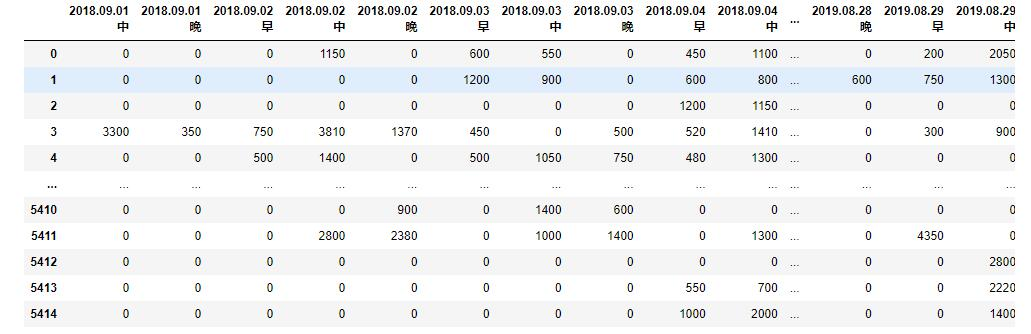
\includegraphics[width=\textwidth]{attachment1_disredundented.jpg}
    \caption{附件一}
    \label{attachment1}
  \end{subfigure}
  \hfill
  \begin{subfigure}[b]{0.3\textwidth}
    \centering
    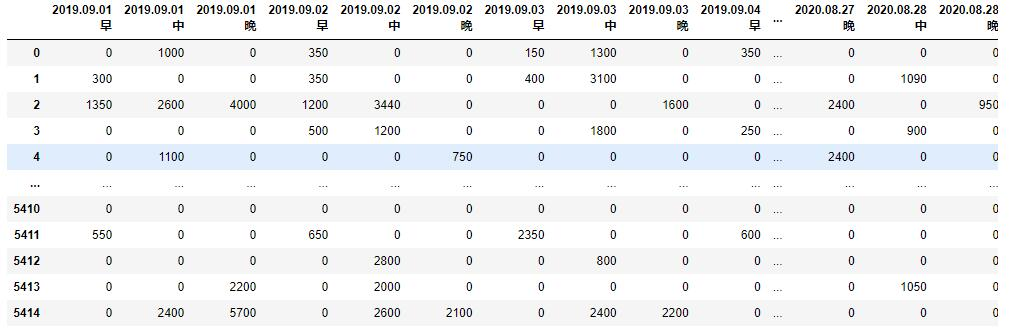
\includegraphics[width=\textwidth]{attachment2_disredundented.jpg}
    \caption{附件二}
    \label{attachment2}
  \end{subfigure}
  \hfill
  \begin{subfigure}[b]{0.3\textwidth}
    \centering
    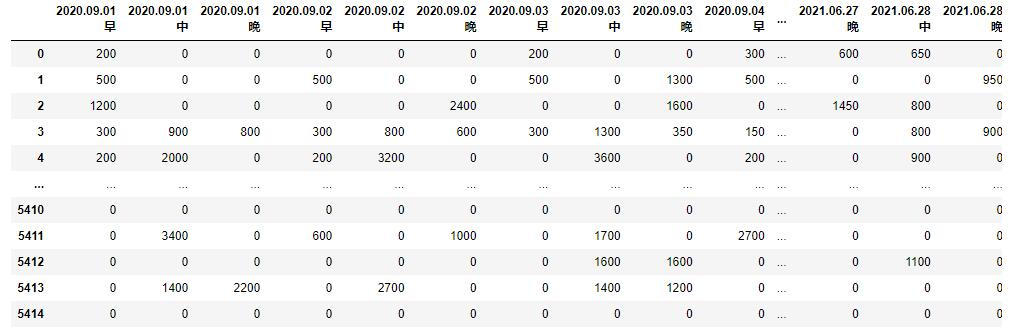
\includegraphics[width=\textwidth]{attachment3_disredundented.jpg}
    \caption{附件三}
    \label{attachment33}
  \end{subfigure}
  \caption{剔除后部分数据}
  \label{attachment1-3}
\end{figure}

\begin{table}[htbp]
  \centering
  \caption{附件1-3剔除的列数}
  \begin{tabular}{ccc}
    \toprule
    学年 & 剔除(列) & 剩余(列) \\
    \midrule
    第一学年 & 73 & 817 \\
    第二学年 & 195 & 417 \\
    第三学年 & 95 & 600 \\
    \bottomrule
  \end{tabular}
\end{table}

从表中可以容易看出,第二学年剔除天数超过一半,不难推出这可能是由于疫情推迟返校所致。

而对于附件4-7,除了一些同学的消费金额外,还提供了他们消费的食物种类。然而,消费食物种类中存在一些缺失值。
鉴于我们已经在附件1-3中有了学生的消费金额数据,显然在这里,消费的食物种类对我们的分析更具价值。
因此,我们决定删除那些消费食物种类为空值的数据。

\subsection{PCA特征提取与数据降维}

为了更好更高效地利用数据,本文通过PCA进行数据降维,找出主成分,避免无效数据对模型的影响。

使用PCA进行数据降维时,我们注意到PCA降维的程度与能量的关系,如图\ref*{dim_num_and_energy}。

\begin{figure}[htbp]
  \centering
  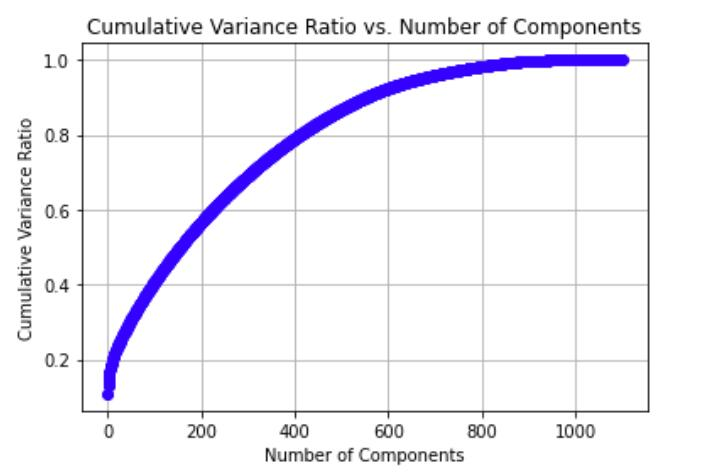
\includegraphics[width=0.8\textwidth]{energy and dim number.png}
  \caption{PCA维度数与能量的关系图}
  \label{dim_num_and_energy}
\end{figure}

主成分数是指在PCA中选择保留的主成分的数量,而能量是指数据在这些主成分上的解释能力。

通常,我们可以通过观察累计解释方差来理解主成分数与能量之间的关系。
累计解释方差表示前n个主成分所解释的总方差比例。随着主成分数的增加,累计解释方差也会增加,
表示所选择的主成分能够解释更多的数据变异性。\cite{reference10}

当我们选择更多的主成分时,能量也会相应增加。因为每个主成分都会贡献一定比例的解释方差,
因此随着维度数的增加,所选择的维度能够解释的数据变异性也会增加。

一般来说,我们希望保留足够数量的维度,以解释大部分的数据能量。通过观察累计解释方差曲线,
我们可以确定保留多少维度才能满足我们的需求。通常,当累计解释方差达到一个可接受的阈值时,
我们可以选择相应的维度数作为数据降维的目标。

考虑到维度数与能量之间的相关关系,这具体取决于数据集的特点和降维的需求。故本文考虑维度为5,
进行PCA降维后得到图像如图。

降维后的数据维度: $(5415, 27)$

每个主成分的累计方差贡献:$[0.11143, 0.13413, 0.14836, \dots, 0.24970, 0.25247, 0.25519]$

\section{基于K-Means聚类算法的学生群体挖掘}

\subsection{K-Means聚类算法}

K-means聚类算法是一种常用的无监督学习算法,用于将数据集分成K个不同的簇(cluster)。它通过最小化样本点与所属簇中心的距离来确定簇的划分。

\subsubsection{算法步骤}

K-means算法的步骤如下:

\begin{enumerate}
  \item 初始化:选择K个初始的聚类中心点。
  \item 聚类分配:对每个样本点,根据其与各个聚类中心的距离,将其分配到最近的簇中。
  \item 更新聚类中心:对每个簇,计算其内部样本点的均值,更新聚类中心。
  \item 重复步骤2和步骤3,直到满足停止条件(如聚类中心不再变化)。
\end{enumerate}

\subsubsection{目标函数和函数意义}

K-means算法的目标函数是最小化所有样本点与其所属簇中心的距离的平方和。定义目标函数$J$如下:

\[
J = \sum_{i=1}^{N} \sum_{j=1}^{K} ||x_i - \mu_j||^2
\]

其中,$x_i$表示第$i$个样本点,$\mu_j$表示第$j$个簇的中心点,$N$表示样本总数,$K$表示簇的数量。

函数意义:目标函数$J$衡量了聚类结果的紧密程度,我们希望通过调整聚类中心,使目标函数最小化,从而得到较好的聚类效果。

\subsubsection{流程图}

下面是K-means聚类算法的流程图:

\begin{figure}[htbp]
  \centering
  \begin{tikzpicture}[node distance=2cm, 
    startstop/.style={rectangle, rounded corners, minimum width=0.8cm, minimum height=0.25cm, text centered, draw=black, fill=red!30}, 
    process/.style={rectangle, minimum width=0.8cm, minimum height=0.25cm, text centered, draw=black, fill=orange!30},
    arrow/.style={thick,->,>=stealth}]

    \node (start) [startstop] {开始};
    \node (init) [process, below of=start] {初始化聚类中心};
    \node (assign) [process, below of=init] {分配样本点到簇};
    \node (update) [process, below of=assign] {更新聚类中心};
    \node (stop) [startstop, below of=update] {停止条件满足};
    \node (end) [startstop, below of=stop] {结束};

    \draw [arrow] (start) -- (init);
    \draw [arrow] (init) -- (assign);
    \draw [arrow] (assign) -- (update);
    \draw [arrow] (update) -- (stop);
    \draw [arrow] (stop) -- node[anchor=east] {是} (end);
    \draw [arrow] (stop.east) -- ++(1.5cm,0cm) |- node[anchor=south] {否} (assign.east);

  \end{tikzpicture}
  \caption{K-Means聚类算法流程图}
  \label{fig:kmeans-flowchart}
\end{figure}

\subsection{聚类结果}

在本文首先采用PCA对原始数据进行特征提取,
提取了5个主成分作为新的特征表示。这一步骤减少了原始数据的维度,同时保留数据中最具代表性和区分性的特征。

接下来,我们将使用K-Means聚类算法对这5个特征进行聚类分析。K-Means算法是一种常用的无监督学习方法,
能够将数据样本划分为K个不同的簇。我们直接以这5个特征作为维度进行聚类,并获得聚类结果。
然后,针对每两个特征的组合,我们分别绘制对应的聚类结果图。通过这种方式,我们可以更好地了解每对特征对聚类结果的影响。

通过K-Means聚类算法,我们得到了一张聚类图。该图展示了在选择不同的特征组合作为维度时,
数据样本的聚类结果。聚类图可以帮助我们观察和分析不同特征组合对于数据聚类的效果,
并从中提取有关数据结构和相似性的信息。\cite{reference1,reference3}

另外,需要注意的是,当数据维度更高时,模型有能力充分学习到多维特征之间的关系。
高维特征提供了更多的信息和表达能力,使得模型能够更好地捕捉数据的复杂性和非线性关系。

然而,随着维度的增加,也面临着所谓的“维度灾难”问题。
高维空间中数据的稀疏性会增加,导致训练数据稀缺以及模型过拟合的风险增加。
因此,在处理高维数据时,我们需要采取一些有效的特征选择、降维或正则化等方法,以提高模型的泛化能力和性能。

\begin{figure}[htbp]
  \centering
  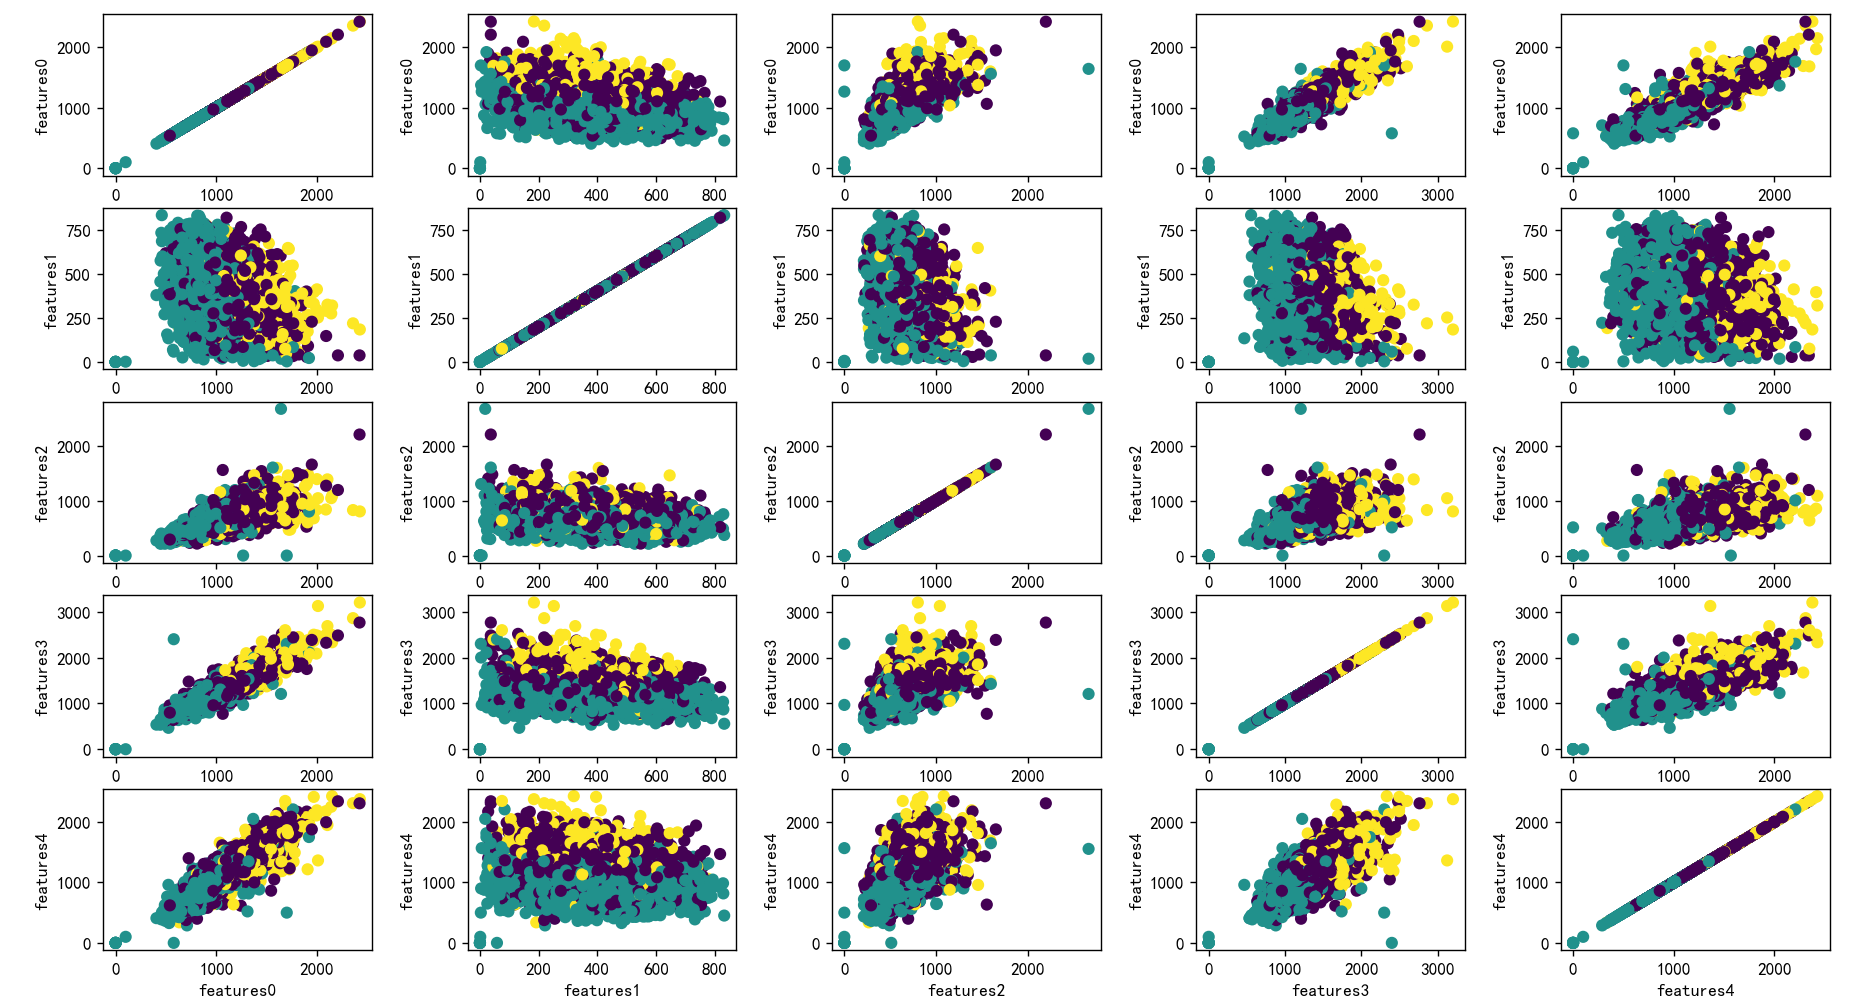
\includegraphics[width=0.8\textwidth]{pca result.png}
  \caption{聚类结果}
  \label{Clustering_result}
\end{figure}

\section{基于XGBoost模型预测学生贫困程度}

\subsection{XGBoost模型}

\subsubsection{模型概念定义}
XGBoost模型是一个集成学习模型,由多个弱分类器组成。每个弱分类器是一棵决策树,它们按顺序逐步提升整体模型的性能。XGBoost使用梯度提升算法来训练这些决策树。\cite{reference7}

\subsubsection{预测函数}
给定一个输入样本$x$,XGBoost模型的预测函数定义如下:
\[
\hat{y}_i = \phi(x_i) = \sum_{k=1}^{K} f_k(x_i)
\]
其中,$\hat{y}_i$表示对样本$x_i$的预测输出,$K$表示决策树的数量,$f_k$表示第$k$棵决策树的预测输出。

\subsubsection{损失函数}
XGBoost使用自定义的损失函数来衡量预测值与真实值之间的差异。常用的损失函数包括平方损失函数(Squared Loss)、
对数损失函数(Logistic Loss)等。损失函数用于构建目标函数。

\subsubsection{目标函数}
XGBoost模型的目标函数由两部分组成:训练数据的损失函数和正则化项。目标函数的定义如下:
\[
\mathcal{L}(\phi) = \sum_{i} l(\hat{y}_i, y_i) + \sum_{k} \Omega(f_k)
\]
其中,$\mathcal{L}(\phi)$表示目标函数,$l(\hat{y}_i, y_i)$表示损失函数,$\Omega(f_k)$表示正则化项,
用于控制模型的复杂度。

\subsubsection{最小化优化的过程}
XGBoost使用梯度提升算法来最小化目标函数。它通过迭代优化决策树的结构和参数,
以降低目标函数的值。优化的过程如下:

\begin{enumerate}
  \item 初始化模型,设定初始决策树的结构和参数。
  \item 逐个决策树进行优化,每次优化都是在当前模型的基础上进行。
  \item 对每个决策树,计算当前模型对训练样本的负梯度(损失函数的一阶导数)作为残差。
  \item 使用残差作为目标值,训练一个新的决策树。采用贪心算法选择最佳的分割点,并更新决策树的叶节点。
  \item 更新模型,将新生成的决策树添加到当前模型中,以减少目标函数的值。
  \item 重复步骤3至5,直到达到预定的迭代次数或目标函数的值收敛。
\end{enumerate}

\subsubsection{目标函数的转化}
在XGBoost中,目标函数由两部分组成:训练数据的损失函数和正则化项。假设损失函数为$l(\hat{y}_i, y_i)$,
正则化项为$\Omega(f_k)$,目标函数表示为$\mathcal{L}(\phi)$。其中,$\hat{y}_i$表示对样本$x_i$的预测输出,
$y_i$表示样本$x_i$的真实值,$f_k$表示第$k$棵决策树的预测输出。

目标函数的转化基于二阶泰勒展开,其核心思想是通过近似原始目标函数的二阶导数项,将目标函数转化为一个更简单的形式。
具体来说,通过对损失函数$l(\hat{y}_i, y_i)$进行二阶泰勒展开,可以得到以下近似形式:
\[
\mathcal{L}(\phi) \approx \sum_{i} \left[ l(\hat{y}_i, y_i) + g_i f_k(x_i) + \frac{1}{2} h_i f_k^2(x_i) \right] + \Omega(f_k)
\]
其中,$g_i$表示损失函数的一阶导数(梯度),$h_i$表示损失函数的二阶导数(二阶梯度)。

通过近似转化后的目标函数,可以简化计算过程。一方面,它将目标函数拆分为每个样本的损失函数项、
一阶导数项和二阶导数项的求和,使得可以针对每个样本进行并行计算。另一方面,
它还将目标函数表示为每棵决策树的预测输出和模型复杂度的和,这样可以使用正则化项对模型进行约束,
控制模型的复杂度,进而防止过拟合。\cite{reference8}

通过目标函数的转化,XGBoost可以更高效地计算目标函数的梯度和二阶导数,并利用这些信息来优化模型。
同时,这种转化也为后续的特征选择、决策树节点分裂等步骤提供了基础。

\subsection{模型优化}

\subsubsection{交叉验证法}

\subsubsection*{模型交叉验证的基本思想}
模型交叉验证的基本思想是将数据集划分为$k$个互斥的子集,通常称为$k$折交叉验证。每次将其中一个子集作为验证集,其余$k-1$个子集作为训练集,进行模型的训练和验证。重复这个过程$k$次,每次使用不同的子集作为验证集,最终得到$k$个模型的性能评估结果。通过对这$k$个结果进行平均,可以得到模型在整个数据集上的性能估计。

\subsubsection*{二分类问题的几种情况}
在二分类问题中,可以根据预测结果和真实标签的组合,将样本分为四种情况:真正例(True Positive, TP)、假反例(False Negative, FN)、假正例(False Positive, FP)和真反例(True Negative, TN)。

\subsubsection*{准确率和召回率的计算}
准确率(Accuracy)和召回率(Recall)是衡量分类模型性能的重要指标。

准确率表示模型预测正确的样本数占总样本数的比例,计算公式如下:
\[
\text{准确率} = \frac{{TP + TN}}{{TP + TN + FP + FN}}
\]

召回率表示模型正确预测为正例的样本数占真实正例样本数的比例,计算公式如下:
\[
\text{召回率} = \frac{{TP}}{{TP + FN}}
\]

\subsubsection*{F1 Score的定义}
F1 Score综合考虑了准确率和召回率,是一个综合评价指标。它是准确率和召回率的调和平均数,计算公式如下:
\[
F1 = \frac{{2 \times \text{准确率} \times \text{召回率}}}{{\text{准确率} + \text{召回率}}}
\]

F1 Score的取值范围为0到1,越接近1表示模型的性能越好。

\subsubsection*{在XGBoost模型上的应用}
对于XGBoost模型,可以在交叉验证过程中,根据不同的性能指标(如准确率、召回率、F1 Score)进行模型的选择和调优。在每个折(fold)的训练和验证过程中,可以计算相应的性能指标,并根据需要选择最佳的模型参数,以提高模型的性能和泛化能力。

具体地,可以在每个折的验证集上计算准确率、召回率和F1 Score,并根据具体问题的要求选择合适的指标进行模型选择和调优。例如,如果重视正例的识别能力,则可以选择召回率作为评价指标,并调整模型参数以提高召回率。如果注重模型的整体性能,则可以选择F1 Score作为评价指标,并优化模型以提高F1 Score的值。\cite{reference9}

通过在交叉验证过程中应用准确率、召回率和F1 Score等指标,可以有效评估和优化XGBoost模型的性能,提高模型在实际应用中的效果。

\subsubsection{启发式算法优化模型参数}

启发式算法可用于优化XGBoost模型参数,以提高模型的性能和准确性。
然而,寻找最佳参数组合的过程是一个复杂的优化问题。在这种情况下,传统的网格搜索方法可能会面临搜索空间过大和计算复杂度高的问题。
这时,启发式算法就发挥了重要作用。
启发式算法通过模拟生物进化、物理粒子运动等自然现象的过程,以非确定性的方式搜索参数空间。
常用的启发式算法包括遗传算法、粒子群优化算法、模拟退火算法等。
这些算法通过不断迭代和优化,逐步接近或达到最优解。\cite{reference4}

在优化XGBoost模型参数时,本文采用启发式算法来搜索参数空间,并评估每个参数组合对模型性能的影响。
算法会根据预定义的目标函数(如交叉验证误差或损失函数)对参数进行调整和更新,直到找到最佳参数组合。
启发式算法具有良好的全局搜索能力和自适应性,能够快速找到近似最优解。
它们在寻找XGBoost模型参数的最佳组合时能够提供更高的效率和准确性。

\subsection{模型预测 —— 贫困等级预测}

本文使用vlookup函数从附件1-3中的特征数据中,查找附件8中部分同学的第一学年的各个特征数据。
同时,在附件9中也使用vlookup函数从附件1-3中的特征数据中查找附件9部分同学的特征。

随后,利用附件8的数据,已知各个指标的特征数据以及贫困等级,
通过训练XGBoost模型并应用启发式算法进行参数寻优,
获得如下最佳参数:学习率为0.2,最大深度为2,弱学习器的数量为50。

各个特征对应的重要性如图\ref{importance_features}:

\begin{figure}[htbp]
  \centering
  \begin{tikzpicture}[scale=1.2]
  \begin{axis}[
      ybar,
      bar width=0.2cm,
      xlabel={特征},
      ylabel={特征重要性},
      ymin=0,
      ymax=0.3,
      xtick=data,
      xticklabels={1,2,3,4,5,6,7,8,9,10,11,12,13,14,15,16,17,18,19,20,21,22,23,24,25,26,27},
      xticklabel style={rotate=90, font=\tiny},
      enlarge x limits=0.2,
      enlarge y limits=0.1,
      legend style={at={(0.5,-0.15)},anchor=north,legend columns=-1},
      area legend
  ]
  \addplot[fill=blue!30] coordinates {
      (1,0.111) (2,0.134) (3,0.148) (4,0.161) (5,0.170) (6,0.179)
      (7,0.185) (8,0.191) (9,0.196) (10,0.200) (11,0.204) (12,0.208)
      (13,0.212) (14,0.215) (15,0.219) (16,0.222) (17,0.226) (18,0.229)
      (19,0.232) (20,0.235) (21,0.238) (22,0.241) (23,0.244) (24,0.247)
      (25,0.250) (26,0.252) (27,0.255)
  };
  \end{axis}
  \end{tikzpicture}
  \caption{特征重要性}
  \label{importance_features}
\end{figure}

而本文相关评价指标如表\ref{performance_XGBoost},其中数据分为三类,标记为0、1、2。

\begin{table}[htbp]
  \centering
  \caption{XGBoost模型评价指标}
  \label{performance_XGBoost}
  \begin{tabular}{cccc}
    \toprule
              & Precision & Recall & F1 Score \\
    \midrule
    0         & 0.79      & 1.00   & 0.83 \\
    1         & 0.86      & 0.02   & 0.02 \\
    2         & 0.71      & 0.00   & 0.02 \\
    Accuracy  &           &        & 0.74 \\
    Average   & 0.79      & 0.76   & 0.65 \\
    \bottomrule
  \end{tabular}
\end{table}

然后本文利用训练好的模型对附件9中的数据进行了预测。但是从结果可以看出,该模型对于贫困等级为“1”、“2”的预测不准确,
这很有可能是因为用于训练的附件8中的标签“1”、“2”太少,导致模型无法进行有效训练。

\subsection{模型改进}

在附件4-7中的301位学生中,有249位学生的信息在附件8中,而另外51位学生的信息在附件9中。
因此,我们将合并后的数据分为两部分。我们从附件8中提取了这249位学生的贫困等级信息,
并使用这些数据训练了XGBoost模型。接下来,我们将使用该模型对另外51位学生的贫困等级进行预测。

然后得到优化后的模型参数:学习率为0.1, 最大深度为2 弱学习器的数量为50。

改进之后重新计算特征重要性,得到图\ref{importance_features_modified}。

\begin{figure}[htbp]
  \centering
  \begin{tikzpicture}[scale=1.2]
  \begin{axis}[
      ybar,
      bar width=0.2cm,
      xlabel={特征},
      ylabel={特征重要性},
      ymin=0,
      ymax=0.3,
      xtick=data,
      xticklabels={1,2,3,4,5,6,7,8,9,10,11,12,13,14,15,16,17,18,19,20,21,22,23,24,25,26,27},
      xticklabel style={rotate=90, font=\tiny},
      enlarge x limits=0.2,
      enlarge y limits=0.1,
      legend style={at={(0.5,-0.15)},anchor=north,legend columns=-1},
      area legend
  ]
  \addplot[fill=blue!30] coordinates {
      (1,0.103) (2,0.126) (3,0.143) (4,0.150) (5,0.172) (6,0.183)
      (7,0.190) (8,0.191) (9,0.199) (10,0.200) (11,0.207) (12,0.208)
      (13,0.214) (14,0.215) (15,0.219) (16,0.222) (17,0.226) (18,0.229)
      (19,0.232) (20,0.234) (21,0.236) (22,0.241) (23,0.246) (24,0.249)
      (25,0.253) (26,0.261) (27,0.273)
  };
  \end{axis}
  \end{tikzpicture}
  \caption{改进后特征重要性}
  \label{importance_features_modified}
\end{figure}

根据表格\ref{performance_XGBoost_modified}结果,可以观察到在引入新的特征后,模型的性能得到了显著提升。
新的模型的准确率为0.86,相比之前的0.74提高了16.22\%。
更为重要的是,新模型对于贫困等级为"1"和"2"的样本的预测准确率有了显著的改善。
原先的模型在对"1"和"2"贫困等级的预测中的F1得分仅为0.02和0.02,而改进后的模型分别达到了0.33和0.67,
提高了数十倍。

\begin{table}[htbp]
  \centering
  \caption{改进后XGBoost模型评价指标}
  \label{performance_XGBoost_modified}
  \begin{tabular}{cccc}
    \toprule
              & Precision & Recall & F1 Score \\
    \midrule
    0         & 0.81      & 1.00   & 0.90 \\
    1         & 1.00      & 0.31   & 0.33 \\
    2         & 1.00      & 0.52   & 0.67 \\
    Accuracy  &           &        & 0.86 \\
    Average   & 0.94      & 0.86   & 0.77 \\
    \bottomrule
  \end{tabular}
\end{table}

\subsection{基于熵权法的贫困等级综合评价}

\subsubsection{熵权法介绍}

熵权法是一种多指标综合评价方法,用于确定各指标在决策过程中的权重。它基于信息熵的概念,通过计算指标的信息熵和差异系数来确定权重,进而计算综合评价值。\cite{reference2}

\textbf{1. 数据标准化}

首先,对原始数据进行标准化处理,将各指标的数据转化为无量纲的相对指标值。
常用的标准化方法包括极差法、标准差法等。

\textbf{2. 信息熵的计算}

对标准化后的数据,计算每个指标的信息熵。
信息熵表示了指标的信息量和不确定性程度。信息熵的计算公式为:

\[
E(X) = -\sum_{i=1}^{n} P_i \log_2(P_i)
\]

其中,\(E(X)\)为指标的信息熵,\(P_i\)为指标在各水平上的概率。

\textbf{3. 差异系数计算}

计算每个指标的差异系数,用于衡量指标的波动程度。差异系数的计算公式为:

\[
CV_i = \frac{{s_i}}{{\bar{x}_i}} \times 100\%
\]

其中,\(CV_i\)为指标的差异系数,\(s_i\)为指标的标准差,\(\bar{x}_i\)为指标的平均值。

\textbf{4. 权重计算}

根据指标的信息熵和差异系数,计算每个指标的权重。权重的计算公式为:

\[
W_i = \frac{{E_i}}{{\sum_{i=1}^{m} E_i + \sum_{i=1}^{m} CV_i}}
\]

其中,\(W_i\)为指标的权重,\(E_i\)为指标的信息熵,\(CV_i\)为指标的差异系数。

\textbf{5. 综合评价值的计算}

最后,根据各指标的权重,计算综合评价值。综合评价值的计算公式为:

\[
V_i = \sum_{i=1}^{m} W_i \times X_i
\]

其中,\(V_i\)为综合评价值,\(W_i\)为指标的权重,\(X_i\)为指标的标准化值。

熵权法通过对数据标准化、信息熵的计算、差异系数的计算、权重的计算和综合评价值的计算,
可以综合考虑各指标之间的重要性和差异性,得出综合评价结果。

\subsubsection{熵权法评分}

本文首先判定了各个特征指标对于贫困程度的正负性,发现本文所提取的特征指标都是正向的,即贫困等级越高,值就越高。
所以如果得到的评价分数越高,学生的贫困等级也就越高。

然后本文对特征指标进行标准化处理,再利用熵权法计算权重。结果如表\ref{weights}。

\begin{table}[htbp]
  \centering
  \caption{指标权重}
  \label{weights}
  \begin{tabular}{cccc}
    \toprule
    feature index  & 信息熵值 & 信息效用值 & 权重(\%) \\
    \midrule
    1         & 0.983     & 0.001  & 0.532 \\
    2         & 0.954     & 0.001  & 0.765 \\
    3         & 0.963     & 0.002  & 0.625 \\
    4         & 0.996     & 0.001  & 0.575 \\
    5         & 1.000     & 0.002  & 0.952 \\
    6         & 0.999     & 0.002  & 1.665 \\
    7         & 0.998     & 0.031  & 4.458 \\
    8         & 1.00      & 0.025  & 4.512 \\
    9         & 1.00      & 0.051  & 5.526 \\
    \dots     & \dots     & \dots  & \dots \\
    \bottomrule
  \end{tabular}
\end{table}

最后,得出全体学生的贫困程度评分,部分结果如表\ref{rates}。

\begin{table}[htbp]
  \centering
  \caption{贫困程度评分}
  \label{rates}
  \begin{tabular}{cccc}
    \toprule
    序号  & 综合评价 & 排名 \\
    \midrule
    5058         & 0.983     & 1     \\
    4962         & 0.976     & 2     \\
    1275         & 0.935     & 3     \\
    5040         & 0.925     & 4     \\
    5107         & 0.923     & 5     \\
    5110         & 0.904     & 6     \\
    4973         & 0.896     & 7     \\
    4918         & 0.883     & 8     \\
    \dots        & \dots     & \dots \\
    \bottomrule
  \end{tabular}
\end{table}

\subsubsection{使用线性插值做资助分配}

为了确保所有80位同学都能获得一定的资助,本文首先确定每位同学的资助额度为625元,总计为625 * 80 = 50000元。
剩下的50000元我们采用线性插值的方法根据学生的贫困程度评分进行分配,以得到每位同学能够获得的额外资助金额。

使用线性插值方法在资助金额分配中有其合理性。
首先,我们知道线性插值是一种简单而常用的插值方法,它基于已知值之间的线性关系来预测未知值。
在资助金额分配中,我们使用学生的贫困程度评分作为已知值,而资助金额作为未知值。
通过线性插值,我们可以根据学生的贫困程度评分来推测其应该获得的资助金额。
其次,线性插值方法具有可解释性和公平性。
通过线性插值,高评分的学生将获得更多的资助金额,这与其贫困程度的评估相符。
这种分配方式基于线性关系,可以较好地反映学生的实际需求,确保资助金额与贫困程度的差异相匹配。
这样的分配方式既公平又符合常识,因为在实际生活中,贫困程度较高的学生通常需要更多的资助来满足基本生活和学习需求。
最后一点,线性插值方法简单易用,计算效率高,适用于大规模数据集和实时决策。
它不需要复杂的参数调整或训练过程,而是根据已知数据进行线性推测,因此具有较低的计算成本和实施难度。

最终得到的结果如下表\ref{allocation}。贫困程度排名第一的同学资助额度为2537元,第80的同学资助额度为200元,且满足总资助金额为100000元。

\begin{table}[htbp]
  \centering
  \caption{资助分配表}
  \label{allocation}
  \begin{tabular}{cccc}
    \toprule
    序号      & 综合评价 & 排名     & 资助金额 \\
    \midrule
    5058      & 0.983     & 1      & 2537  \\
    4962      & 0.976     & 2      & 2483  \\
    1275      & 0.935     & 3      & 2356  \\
    5040      & 0.925     & 4      & 2309  \\
    5107      & 0.923     & 5      & 2293  \\
    \dots     & \dots     & \dots  & \dots \\
    4966      & 0.635     & 77     & 336   \\
    5038      & 0.612     & 78     & 305   \\
    5082      & 0.607     & 79     & 267   \\
    5068      & 0.594     & 80     & 200   \\
    \bottomrule
  \end{tabular}
\end{table}

\subsubsection{方案合理性分析}

为验证模型合理性,我们在给出的基础数据基础上进行整合以及统计量的提取,
分别得到日均消费、消费最高值、消费极差(最大值-最小值)、全年消费方差、日消费方差、上四分位点、下四分位点,
并且利用这些指标对于模型效果进行评估,以验证我们的模型选取真正需要资助的贫困学生,从统计意义上得到了一个性能良好的隐性资助模型。

\begin{table}[htbp]
  \centering
  \caption{选出的80位同学与附件8中的贫困群体特征对比}
  \label{comparison}
  \begin{tabular}{ccccc}
    \toprule
    指标 & 贫困程度0 & 贫困程度1 & 贫困程度2 & 贫困评分前80 \\
    \midrule
    次消费均价      & 987     & 965      & 973    & 930  \\
    最高值          & 4689    & 4786    & 3962    & 4496 \\
    消费极差        & 4495    & 4537     & 3920   & 4382 \\
    全年消费波动性  & 593     & 580      & 648    & 586  \\
    日消费波动性    & 435     & 432     & 428     & 480  \\
    上四分位点      & 1285    & 1137     & 1159   & 1092 \\
    下四分位点      & 723     & 697      & 702    & 664  \\
    \bottomrule
  \end{tabular}
\end{table}

使用熵权法综合评价学生贫困程度并分配资助金额,采用线性插值算法进行分配。
贫困程度高的学生获得更多资助,而贫困程度低的学生获得较少资助,同时设置最小资助额度以确保每位获得资助的学生都能得到一定帮助。
这种方法公平地考虑了学生的贫困程度,符合教育资助的目标。

\section{模型改进}

\subsection{模型优点}
\begin{itemize}
  \item 在进行特征提取时,我们充分挖掘了数据特征,利用主成分分析法从附件1-3和4-7两个数据集中提取了多个指标,减少了模型的过拟合可能。
  \item 对于聚类算法,我们通过分析聚类结果关于两两特征的分布,以帮助我们发现数据中的内在模式和关联关系。通过聚类算法的应用,我们能够将相似特征的样本归为一类,为模型提供更具区分性的信息。
  \item 在构建XGBoost模型时,我们还采用了多种方法来进一步提高模型的准确度。其中,交叉验证被用于评估模型的泛化性能和确定合适的参数配置,而启发式算法寻优则帮助我们在参数空间中搜索最佳的模型配置,以使模型能够更好地适应数据的特点。
  \item 为了确保资助金额的公平分配,我们运用了熵权法进行综合评价和线性插值的方式。通过熵权法,我们能够综合考虑多个评价指标的重要性,以更准确地评估学生的贫困程度。同时,我们遵循公平性和差异化原则,采用线性插值方法在资助金额的分配上实现公平和差异化,以更好地满足教育资助的目标。
  \item 这些措施的综合运用不仅使我们能够准确地揭示学生的贫困程度,还充分体现了公平性和差异化原则,为教育资助工作提供了有力支持。我们的研究旨在确保对每个学生的需求给予关注,同时提高教育资助的准确性和效率。
\end{itemize}

\subsection{模型缺点}
\begin{itemize}
  \item 附件8中贫困等级为1和2的数据较少,导致XGBoost模型在识别这两类贫困等级时不准确。
  \item 此外,附件4-7仅提供了300位同学的消费食物种类数据,无法代表所有同学的情况。因此,即使我们通过这300位同学的数据训练出优化后的模型,也无法对其他同学进行准确的预测。
  \item 尽管学生的餐厅消费数据在很大程度上反映了他们的贫困程度,但它无法全面揭示所有方面。例如,学生的出行方式也可反映经济状况。不同出行方式对学生的经济负担影响不同,如使用公共交通工具相对于自驾车更经济实惠。因此,未来研究可以探索学生的出行方式数据及其他相关指标,以更全面、准确评估学生的贫困程度。这将提高贫困等级预测模型的精度和适用性,并帮助确定学生的经济援助需求。
\end{itemize}

\subsection{模型改进策略}
\begin{itemize}
  \item 引入领域专家知识:与专家合作,利用其领域知识和经验来指导模型的构建和优化。专家可以提供有关贫困特征的洞察和指导,帮助确定关键指标、权重和算法选择,从而提高模型的准确性和解释性。
  \item 使用集成学习方法:尝试集成多个不同算法的预测结果,如随机森林、梯度提升树等。通过结合不同算法的预测能力,可以减少单个算法的偏差和方差,提高整体模型的性能和稳定性。
  \item 优化数据预处理:仔细审查和处理数据中的缺失值、异常值和噪声等问题。采用合适的数据清洗和处理技术,如插补缺失值、平滑异常值等,可以改善数据质量,从而提高模型的准确性和稳定性。
  \item 精细化权重确定方法:在使用熵权法进行综合评价时,权重的确定对模型的准确性至关重要。除了基于数据的信息熵确定权重外,可以考虑采用基于专家经验或机器学习的方法来确定权重。专家经验提供领域知识和直觉,而机器学习方法可以通过学习数据模式来确定权重,从而更准确地反映指标对评价结果的真实影响。
  \item 通过采用这些优化手段,可以不断改进隐性资助模型,提高其预测准确性、稳定性和实用性,从而更好地为经济困难学生提供精准的教育援助。
\end{itemize}

\newpage

% References
\begin{thebibliography}{9}
% Your bibliography entries here
\bibitem{reference1} Zhou, J., Wu, J., Hong, J., et al. (2014). \textit{ An Entropy Weighting K-Means Algorithm for Robust Subspace Clustering}. Information Sciences, 258, 342-359.
\bibitem{reference2} Zhu, C., Xu, Z.S., Liu, S. (2018).\textit{An Entropy Weighting Multi-Granular Fuzzy Decision-Making Method Based on Multi-Dimensional Uninorms}. Information Sciences, 429, 102-121.
\bibitem{reference3} Hartigan, J. A., Wong, M. A. (1979). \textit{Algorithm AS 136: A K-Means Clustering Algorithm}. Journal of the Royal Statistical Society: Series C (Applied Statistics), 28(1), 100-108.
\bibitem{reference4} Lloyd, S. P. (1982). \textit{Least Squares Quantization in PCM}. IEEE Transactions on Information Theory, 28(2), 129-137.
\bibitem{reference5} Steinley, D. (2004). \textit{Properties of the Hubert-Arabie Adjusted Rand Index}. Psychological Methods, 9(3), 386-396.
\bibitem{reference6} 郭鹏, 张丽蓉. (2015). 数学建模中的优化问题与方法. 计算机与现代化, (4), 28-30.
\bibitem{reference7} Chen, T., Guestrin, C. (2016). \textit{XGBoost: A Scalable Tree Boosting System. In Proceedings of the 22nd ACM SIGKDD International Conference on Knowledge Discovery and Data Mining (pp. 785-794)}. ACM.
\bibitem{reference8} Friedman, J. H. (2001). \textit{Greedy Function Approximation: A Gradient Boosting Machine}. Annals of Statistics, 29(5), 1189-1232.
\bibitem{reference9} Sokolova, M., Lapalme, G. (2009). \textit{A Systematic Analysis of Performance Measures for Classification Tasks}. Information Processing and Management, 45(4), 427-437.
\bibitem{reference10} Jolliffe, I. T. (2002). \textit{Principal Component Analysis (2nd ed.)}. Springer.
\end{thebibliography}

\newpage

\lstset{basicstyle=\ttfamily}

\section{附录}

支撑材料目录:

adde\_1\_adde\_3\_processing.py

entropy\_weight\_func.py

pca\_dimension\_reduction.py

pca\_painting.py

t1-kmeans.py

t2t3-xgboost.py

附件9\_待补全标签数据\_.xlsx

\appendix % 切换到附录部分

\section{数据处理代码}

\begin{lstlisting}[language=Python]
import pandas as pd
from sklearn.decomposition import PCA
from scipy.stats import f_oneway

pca = PCA(n_components=100)

adde_1 = pd.read_excel('C:\\Users\\Herrywen\\Desktop\\adde_1.xlsx')
adde_2 = pd.read_excel('C:\\Users\\Herrywen\\Desktop\\adde_2.xlsx')
adde_3 = pd.read_excel('C:\\Users\\Herrywen\\Desktop\\adde_3.xlsx')

adde_3 = adde_3.iloc[:,1:]
adde_1 = adde_1.iloc[:,1:]
adde_2 = adde_2.iloc[:,1:]

non_zero_counts = adde_1.astype(bool).sum()
columns_to_drop = non_zero_counts[non_zero_counts < 1000].index
adde_1 =  adde_1.drop(columns_to_drop, axis=1)
adde_1

non_zero_counts = adde_2.astype(bool).sum()
columns_to_drop = non_zero_counts[non_zero_counts < 1000].index
adde_2 =  adde_2.drop(columns_to_drop, axis=1)
adde_2

non_zero_counts = adde_3.astype(bool).sum()
columns_to_drop = non_zero_counts[non_zero_counts < 1000].index
adde_3 =  adde_3.drop(columns_to_drop, axis=1)
adde_3
\end{lstlisting}

\section{PCA数据降维代码}

\begin{lstlisting}[language=Python]
import pandas as pd
from sklearn.decomposition import PCA
import numpy as np
df

# 创建PCA对象
pca = PCA()

# 执行PCA降维
pca.fit(df)

# 计算每个主成分的累计方差贡献
explained_variance_ratio=pca.explained_variance_ratio_

# 计算累计方差贡献的累积和
cumulative_variance_ratio=np.cumsum(explained_variance_ratio)

# 确定保留的主成分个数
n_components=np.argmax(cumulative_variance_ratio >= 0.255)+1

# 根据保留的主成分个数重新执行PCA降维
pca = PCA(n_components=n_components)
reduced_data = pca.fit_transform(df)

# 输出降维后的数据
print("降维后的数据维度:", reduced_data.shape)

# 输出每个主成分的累计方差贡献
print("每个主成分的累计方差贡献:",
cumulative_variance_ratio[:n_components])

# 可选:根据需要,将降维后的数据转换回DataFrame对象
data = pd.DataFrame(reduced_data)

# 创建主成分的序号数组
components = np.arange(1, len(cumulative_variance_ratio) + 1)

# 绘制关系图
plt.plot(components, cumulative_variance_ratio,
marker='o', linestyle='-', color='b')
plt.xlabel('Number of Components')
plt.ylabel('Cumulative Variance Ratio')
plt.title('Cumulative Variance Ratio vs. Number of Components')
plt.grid(True)
plt.show()
\end{lstlisting}

\section{K-Means聚类代码}

\begin{lstlisting}[language=Python]
import pandas as pd
import numpy as np
data = pd.read_csv("D:/wtz_code/shumo/数据集聚类标注.csv")
labels = data["聚类种类"]
from sklearn.cluster import KMeans

# 创建KMeans对象并指定聚类簇的数量,执行K-means聚类
kmeans = KMeans(n_clusters=3)
kmeans.fit(data)

# 获取聚类结果,即每个样本所属的簇标签,获取聚类的中心点
labels = kmeans.labels_
centroids = kmeans.cluster_centers_

# 输出聚类结果和中心点
print("聚类结果:", labels)
print("聚类中心点:", centroids)
import matplotlib.pyplot as plt

# 绘制聚类图
plt.rcParams['font.sans-serif']= ['SimHei']
plt.title('K-means Clustering')
for i in range(n):
    for j in range(n):
        plt.subplot(5,5,5 * j + i + 1 )
        plt.scatter(data[i], data[j], c = labels, cmap='viridis')
        plt.xlabel("features"+str(i))
        plt.ylabel("features"+str(j))
plt.show()
\end{lstlisting}

\section{问题二、三相关代码}

\begin{lstlisting}[language=Python]
import pandas as pd
import xgboost as xgb
from sklearn.model_selection import GridSearchCV
from sklearn.metrics import classification_report
import matplotlib.pyplot as plt
import seaborn as sns

# 加载数据
data_train=pd.read_excel("D:/wtz_code/shumo/附件8 已知贫困标签.xlsx")
data_predict=pd.read_excel("D:/wtz_code/shumo/附件9_待补全标签数据.xlsx")

# 分割特征和标签
X_train = data_train.iloc[:, 2:]
y_train = data_train.iloc[:, 1]
X_test = data_predict.iloc[:, 2:]

# 定义模型
model = xgb.XGBClassifier()

# 定义参数网格
param_grid = {
    'max_depth': [2, 4, 6],
    'n_estimators': [50, 100, 200],
    'learning_rate': [0.01, 0.1, 0.2],
}

# 创建网格搜索对象
grid_search = GridSearchCV(model, param_grid, cv=5, scoring='accuracy')

# 训练模型
grid_search.fit(X_train, y_train)

# 输出最优参数
print("Best parameters: ", grid_search.best_params_)
print("Best score: ", grid_search.best_score_)

# 使用最优模型预测
y_pred = grid_search.predict(X_test)

# 保存预测结果到原数据中
data_predict.iloc[:, 1]=y_pred
data_predict.to_excel("D:/wtz_code/shumo/附件9_待补全标签数据.xlsx",
index=False)

# 输出模型报告
print("Classification report:\n",
classification_report(y_train, grid_search.predict(X_train)))

# 输出特征重要性
feature_importances=grid_search.best_estimator_.feature_importances_
sns.barplot(x=feature_importances, y=X_train.columns)
plt.xlabel('Feature Importance Score')
plt.ylabel('Features')
plt.title("Visualizing Important Features")
plt.show()
\end{lstlisting}

\section{问题四相关代码(熵权法)}

\begin{lstlisting}[language=Python]
import numpy as np
def entropy_weights(matrix):
    # 计算评价指标得分矩阵的行数和列数和评价指标得分矩阵的列归一化矩阵
    m, n = matrix.shape
    normalized_matrix=matrix/np.sum(matrix, axis=0)

    # 计算每个评价指标的信息熵
    entropy=-np.sum(normalized_matrix*np.log2(normalized_matrix), axis=0)

    # 计算每个评价指标的权重
    weights=(1-entropy)/np.sum(1-entropy)

    return weights
\end{lstlisting}

\end{document}
